\section{任务三}
\subsection{实验目标与方法}

本任务对任务一选取的四轮差分
    $\Delta_{\mathrm{in}} = \texttt{0x0001}
    \quad\longrightarrow\quad
    \Delta_{\mathrm{out}} = \texttt{0x0010}$
进行实验验证。随机选取五组不同的轮密钥，在每组密钥下遍历
全部 $2^{16}$ 个明文 $x$，构造满足输入差分为
$\Delta_{\mathrm{in}}$ 的明文对
\[
    (x,x')=(x,x\oplus\Delta_{\mathrm{in}}),
\]
分别进行四轮 CipherFour 加密，统计密文差分等于
$\Delta_{\mathrm{out}}$ 的次数，并计算相应频率及五组频率的平均值。

为使实验结果可以复现，程序使用伪随机数生成器产生轮密钥，
并将随机种子固定为 \texttt{20261001}。每组密钥记为
\[
    K^{(j)}=(K_0^{(j)},K_1^{(j)},K_2^{(j)},K_3^{(j)},K_4^{(j)}),
    \qquad j=1,\ldots,5,
\]
其中每个密钥字均为 16 比特，且五组密钥互不相同。

四轮加密的每一轮均包含轮密钥异或、S 盒替换和 P 置换，
第四轮同样保留 P 置换。设初始状态为 $u_0=x$，则
\[
    u_{r+1}=P\bigl(S(u_r\oplus K_r)\bigr),
    \qquad r=0,1,2,3,
\]
最终密文为
\[
    E_K(x)=u_4\oplus K_4.
\]
其中，$S$ 表示对 16 比特状态的四个半字节并行应用 S 盒。

对于第 $j$ 组密钥，满足目标输出差分的有序明文对数为
\[
    N_j =
    \#\left\{
        x\in\{0,1,\ldots,2^{16}-1\}:
        E_{K^{(j)}}(x)\oplus
        E_{K^{(j)}}(x\oplus\Delta_{\mathrm{in}})
        =\Delta_{\mathrm{out}}
    \right\},
\]
相应的差分出现频率为
\[
    f_j=\frac{N_j}{2^{16}},
\]
五组密钥下的平均频率为
\[
    \overline{f}=\frac{1}{5}\sum_{j=1}^{5}f_j.
\]

本实验采用有序对计数。由于输入差分非零，每个无序明文对
$(x,x')$ 会以 $(x,x')$ 和 $(x',x)$ 两种顺序各计数一次。
若改用无序对计数，则匹配对数与总对数均减半，
因此最终得到的频率不变。

\subsection{程序实现}

程序首先预计算全部 16 比特状态经过 S 盒和 P 置换后的结果，
建立查找表
\[
    \mathrm{SP}[v]=P(S(v)).
\]
加密时，每轮通过查表完成 S 盒替换和 P 置换：
\begin{lstlisting}
state = plainText
for round_index in range(NUMBER_OF_ROUNDS):
    state = SP_table[state ^ keys[round_index]]
return state ^ keys[NUMBER_OF_ROUNDS]
\end{lstlisting}

对于每组密钥，程序先计算全部明文对应的密文，
然后遍历明文 $x$，通过 $x\oplus\Delta_{\mathrm{in}}$
定位配对明文，判断对应的密文差分是否为目标输出差分。
核心统计过程如下：
\begin{lstlisting}
count = 0
for plainText in range(STATE_SIZE):
    paired_plainText = plainText ^ INPUT_DIFFERENCE
    if (
        cipherText[plainText] ^ cipherText[paired_plainText]
        == OUTPUT_DIFFERENCE
    ):
        count += 1

frequency = count / float(STATE_SIZE)
\end{lstlisting}

这种方法对每组密钥均覆盖全部 $2^{16}$ 个明文，
得到该固定密钥下目标差分的实际出现频率。

\subsection{实验结果}

本次实验随机生成的五组轮密钥如
表~\ref{tab:task3_keys} 所示，各组密钥下的匹配对数及频率如
表~\ref{tab:task3_frequency} 所示。表中密钥均采用十六进制表示。

\begin{table}[H]
    \centering
    \caption{任务三使用的五组轮密钥}
    \label{tab:task3_keys}
    \small
    \renewcommand{\arraystretch}{1.2}
    \begin{tabular}{cccccc}
        \toprule
        组别 & $K_0$ & $K_1$ & $K_2$ & $K_3$ & $K_4$ \\
        \midrule
        1 & \texttt{7998} & \texttt{A426} & \texttt{B83F}
          & \texttt{C8AA} & \texttt{3F89} \\
        2 & \texttt{4CC3} & \texttt{605E} & \texttt{27E6}
          & \texttt{45C7} & \texttt{1314} \\
        3 & \texttt{5F96} & \texttt{ECF1} & \texttt{C21E}
          & \texttt{6D7E} & \texttt{AE5A} \\
        4 & \texttt{620C} & \texttt{890A} & \texttt{8237}
          & \texttt{C80D} & \texttt{6808} \\
        5 & \texttt{A00C} & \texttt{0D2F} & \texttt{7645}
          & \texttt{7F31} & \texttt{86AC} \\
        \bottomrule
    \end{tabular}
\end{table}

\begin{table}[H]
    \centering
    \caption{不同密钥下目标输出差分的出现频率}
    \label{tab:task3_frequency}
    \renewcommand{\arraystretch}{1.2}
    \begin{tabular}{ccc}
        \toprule
        组别 & 匹配有序明文对数 $N_j$ & 频率 $f_j$ \\
        \midrule
        1 & 3144 & 0.0479736328 \\
        2 & 3124 & 0.0476684570 \\
        3 & 3120 & 0.0476074219 \\
        4 & 3196 & 0.0487670898 \\
        5 & 3018 & 0.0460510254 \\
        \midrule
        平均 & 3120.4 & 0.0476135254 \\
        \bottomrule
    \end{tabular}
\end{table}

程序运行结果如图~\ref{fig:task3_result} 所示。

\begin{figure}[H]
    \centering
    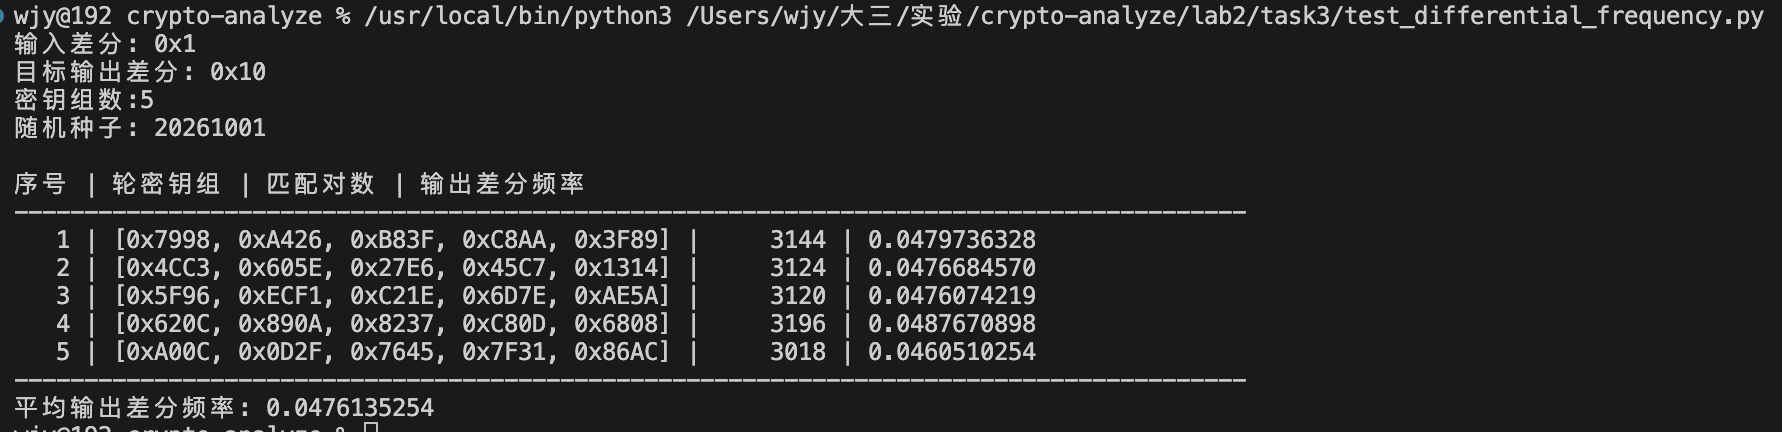
\includegraphics[width=0.95\textwidth]{figures/task3_result.png}
    \caption{五组随机密钥下的四轮差分频率测试结果}
    \label{fig:task3_result}
\end{figure}

五组密钥下的平均频率为
\[
    \overline{f}
    =\frac{3144+3124+3120+3196+3018}{5\times65536}
    =0.047613525390625,
\]
即目标输出差分的平均出现频率约为 $4.7614\%$。

\subsection{结果分析}

按 S 盒差分分布表计算并累加各条差分路线概率，
所选四轮差分的理论概率为
\[
    P_{\mathrm{DDT}}
    =0.0479736328125.
\]
本次实验的平均频率与该理论概率的绝对差为
\[
    \left|\overline{f}-P_{\mathrm{DDT}}\right|
    =0.000360107421875,
\]
相对偏差为
\[
    \frac{\left|\overline{f}-P_{\mathrm{DDT}}\right|}
         {P_{\mathrm{DDT}}}
    \times100\%
    \approx0.7506\%.
\]
可见，本次五组密钥下的平均频率与 DDT 理论概率较为接近。

各组密钥下的频率并不完全相同，其中第四组最高，
约为 $4.8767\%$，第五组最低，约为 $4.6051\%$。
虽然同一轮密钥在一对状态的异或中会抵消，
但轮密钥会改变进入 S 盒的具体取值，
进而影响后续各轮差分传播的实际计数。
因此，固定密钥下的差分频率可以随密钥变化。

DDT 路线概率的乘积及其求和对应独立均匀轮密钥条件下
的平均概率，而本实验仅选取五组具体密钥，
其平均频率不必与理论概率完全相等。
同时，每组密钥下已穷举全部明文，
因此这里的差异不是由明文抽样不充分造成的。

实验结果表明，在本次选取的五组密钥下，
差分 $\texttt{0x0001}\rightarrow\texttt{0x0010}$
均保持较高的出现频率，其平均值与理论计算接近，
为任务一所选高概率差分提供了实验验证。